Prinzipell lässt sich sagen, dass eine Software nur dann für den Endkunden tauglich ist, wenn sie reichlich getestet ist. Hierfür gibt es zahlreiche verschiedene Methoden. Vor einiger Zeit wurde die eigentliche Entwicklung der Software und das testen noch als eigene Prozesse angesehen. Erst mit dem US-amerikanischen Softwareentwickler Kent Beck wurde der Test-First-Ansatz bekannt. Hierbei wird der vorherige Ablauf umgekhert und anstatt mit dem Quellcode zu beginnen schrieb Beck zuerst einen Test und programmierte dann den dazu benötigten Code. Für einen Laien mag die testgetriebene Entwicklung am Anfang wohl eher sinnlos erscheinen. Dennoch ist sie sehr effizient, da somit jedes Feature des Quellcodes mit einem Test abgedeckt ist. Des Weiteren schreiben die Entwickler:innen nur den erforderlichen Code, um sicherzustellen, dass der Test erfolgreich durchgeführt wird. Dadurch wird vermieden, unnötigen Code zu schreiben, der nicht direkt zum Ziel des Tests beiträgt. Diese präzise Vorgehensweise trägt dazu bei, den Testprozess effizienter zu gestalten und sicherzustellen, dass das entwickelte Softwaremodul genau das tut, was es soll, ohne zusätzliche, unnötige Komplexität einzuführen.

\begin{figure}
    \centering
    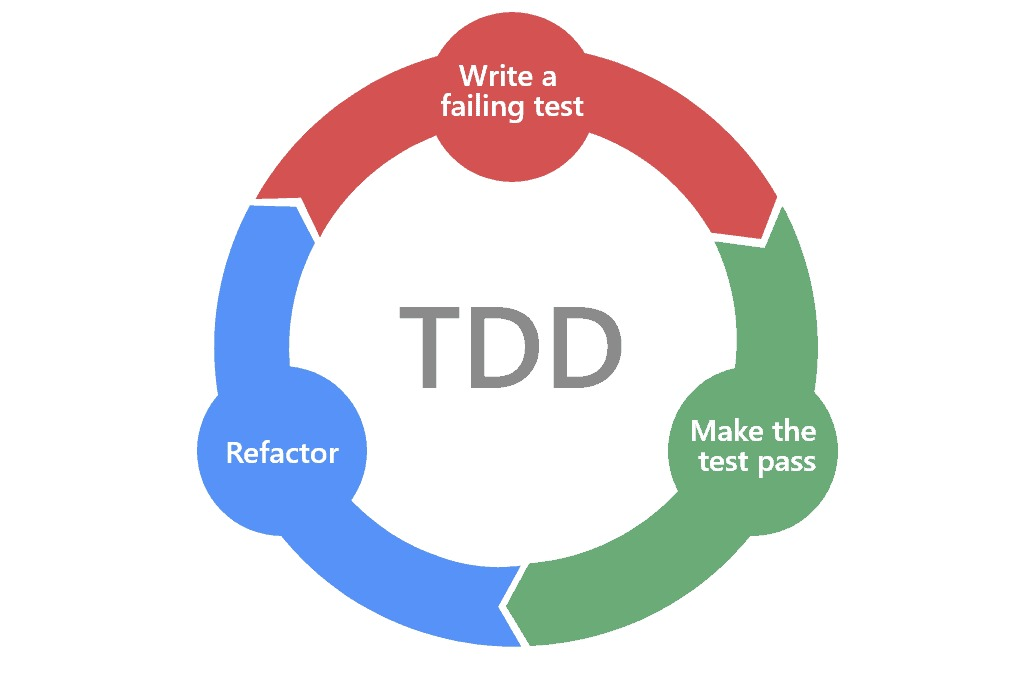
\includegraphics[width=0.5\linewidth]{pics/tdd.jpeg}
    \caption{Wie funktioniert Test Driven Development}
    \label{fig:enter-label}
    \cite{tdd_grafik}
\end{figure}

\subsection{Wie funktioniert Test Driven Developement}

Test Driven Developement (TDD) folgt den Ergebnissen, von den schon im vorhinein definierten Testfällen. Dieser zyklische Ansatz stellt sicher, dass der Code nur in das Produktivsystem gelangt, wenn alle Testanforderungen erfüllt sind und somit keine Fehler mehr auftreten. Das bedeutet, dass der Quellcode so lange überarbeitet wird, bis der Test erfolgreich durchgeführt wird und keine Fehler mehr aufweist. Neue Funktionen werden schrittweise zum Code hinzugefügt, wodurch das Test-driven Development (TDD) zu den inkrementellen Vorgehensweisen in der Softwareentwicklung zählt. Durch diesen iterativen Prozess wird die Software Stück für Stück erweitert und verbessert, wobei jede Iteration auf die vorherigen Schritte aufbaut und das Risiko von Fehlern reduziert wird.

\cite{Was_ist_TDD}

